\documentclass[11pt]{article}


% Use wide margins, but not quite so wide as fullpage.sty
\marginparwidth 0.5in 
\oddsidemargin 0.25in 
\evensidemargin 0.25in 
\marginparsep 0.25in
\topmargin 0.25in 
\textwidth 6in \textheight 8 in
% That's about enough definitions


\usepackage[utf8]{inputenc}
\usepackage{color}
\usepackage{graphicx}
\usepackage{subfig}
\usepackage[backend=bibtex,style=numeric,natbib=true ,bibencoding=ascii]{biblatex} % User the bibtex backend with the authoryear citation style (which resembles APA)

\addbibresource{ref.bib} % The filename of the bibliography
\usepackage{hyperref}

% multirow allows you to combine rows in columns
\usepackage{multirow}
% tabularx allows manual tweaking of column width
\usepackage{tabularx}
% longtable does better format for tables that span pages
\usepackage{longtable}

\begin{document}

\author{Florian J\"org\\Viviane Tanner\\Adrian W\"alchli}

\title{\textbf{Super Resolution \\ Project Report}}
\maketitle



\section{Super Resolution}

Super resolution is a term used to describe methods for image upscaling. Those methods generate a high resolution output from a low resolution input image. To achieve this, missing data has to be interpolated.

It's possible for two different but very similar high resolution images to have the same low resolution image. Therefore super resolution is an ill-posed problem that does not have a unique solution.

Neural networks present an easy way to handle such problems. They learn a probability distribution over inputs and outputs. Because of that they can be reasonably trained even when there are ambiguities.

Furthermore the Super Resolution Neural Network (SRNN) does not have to work on all inputs (e.g. there is no use in upscaling an image that contains only noise). The domain it works on can be significantly reduced, increasing its accuracy. For example a SRNN used in neuroscience only has to be able to upscale pictures of nervous tissue, knowledge about how to upscale faces would be useless to it.

The first to use neural networks for super resolution were \citet{dong2016image}. They only used three convolutional layers. The first extracts low resolution feature maps, the second maps those to high resolution feature maps, and the last reconstructs the high resolution image.
Even this simple network was already able to outperform other state of the art algorithms of that time.

Since then many different SRNNs were proposed. Most fit in one of two categories: They either directly upscale the image (like \citet{dong2016image}) or they use a naive upscale algorithm (e.g. bicubic interpolation) and then try to improve the quality of the intermediate output with a neural network.

\newpage
\section{Proposed Network Architecture}

As can be seen in Figure \ref{label:mainNetworkGraph} and Table \ref{table:main_architecture}, our proposed architecture consists of two parts:
\begin{itemize}
	\item 	Upscaling: Convolutional layers that perform upscaling to the desired image size. 
	\item 	Refinement: A recurrent neural network that adds more detail to the upscaled image in an iterative manner using residual learning.
			
\end{itemize}
With this architecture we attempt to combine both approaches to SRNN currently in use.

\begin{figure}[t]
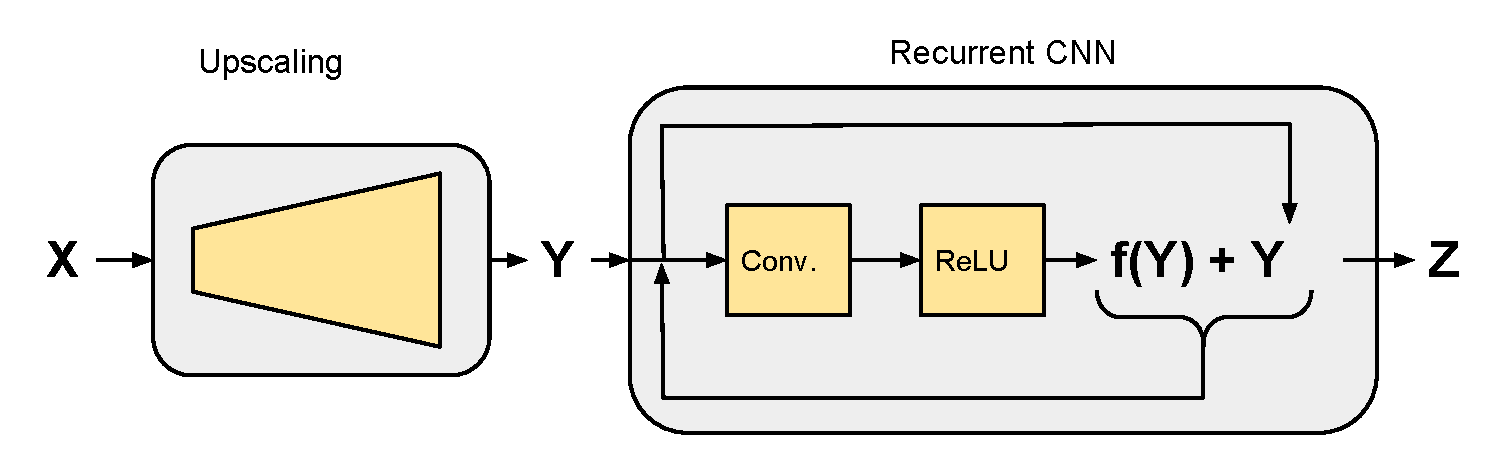
\includegraphics[width=\textwidth]{imgs/MainNet.pdf}
\caption{Our main network}
\label{label:mainNetworkGraph}
\end{figure}
\begin{table}[h!]
    \renewcommand{\arraystretch}{1.5}
    \centering
    \begin{tabular}{ |l|l|l|r|r| }
        \hline
        \textbf{Part} & \textbf{Name} & \textbf{Type} & \textbf{Kernel Size} & \textbf{Out Channels} \\
        \hline
        \multirow{6}{*}{Upscale} & conv1 & Convolution & 3 & 6 \\
        \cline{2-5}
        & conv2 & Convolution & 3 & 6 \\
        \cline{2-5}
        & conv3 & Convolution & 5 & 32 \\
        \cline{2-5}
        & conv4 & Convolution & 3 & $3*upscale^2$ \\
        \cline{2-5}
        & shuffle & PixelShuffle & - & 3\\
        \hline
        \multirow{2}{*}{Recurrent} & conv5 & Convolution & 3 & 6 \\
        \cline{2-5}
        & conv6 & Convolution & 3 & 3 \\
        \hline
    \end{tabular}
    \caption{These are the layers used in our network. There is an additional ReLU layer after each convolutional layer except for conv4. The layers listed in the recurrent part form the inside of the recursion.}
    \label{table:main_architecture}
\end{table}


\subsection{Variations}

We conduct two ablation studies to investigate the impact of our design choices in the network architecture. 
Additionally, we train the full network in two separate steps to understand which part trains and converges faster. 
Finally we tried to make the two parts of the network deeper.

\paragraph{Upscale Only}

In order to find out how effective our refinement network is, we simply remove it and compute the metrics for comparison.
This version of the network is very similar to the one proposed in \citet{dong2016image}.

\paragraph{Omitting the Residual Connection}

The residual part of the network aims to add details to the image that could not be learned by the first part.
By removing it, we expect the network to perform worse in regions where the network should reconstruct texture detail.

\paragraph{Two-Step Training}

When training the full network at once, it could be that the recurrent block has a bad influence on the training of the upscale part.
In order to make sure that this is not the case, we propose to train in two stages.
In the first step, we only train the upscale part as described for the upscale only variation. 
Then, the second part is trained with the weights of the first part fixed.
Finally, we compare the metrics with the other variants.%in tables~\ref{label:tableResultsSet5} and~\ref{label:tableResultsSet100}.

\paragraph{Deeper Network}

With a deeper network, we add complexity to our model and expect the network to learn more variations of detail in the data.
We added two additional convolution layers in the upscale network and one in the refinement part.
The exact layout of the deep network is presented in table~\ref{table:main_architecture_deep}.
In this iteration, we also enlarged the kernel sizes of the first layers.


\begin{table}[h!]
    \renewcommand{\arraystretch}{1.5}
    \centering
    \begin{tabular}{ |l|l|l|r|r| }
        \hline
        \textbf{Part} & \textbf{Name} & \textbf{Type} & \textbf{Kernel Size} & \textbf{Out Channels} \\
        \hline
        \multirow{5}{*}{Upscale} & conv1 & Convolution & 11 & 6 \\
        \cline{2-5}
        & conv2 & Convolution & 7 & 6 \\
        \cline{2-5}
        & conv3 & Convolution & 3 & 12 \\
        \cline{2-5}
        & conv4 & Convolution & 5 & 16 \\
        \cline{2-5}
        & conv5 & Convolution & 3 & 32 \\
        \cline{2-5}
        & conv6 & Convolution & 3 & $3*upscale^2$ \\
        \cline{2-5}
        & shuffle & PixelShuffle & - & 3\\
        \hline
        \multirow{2}{*}{Recurrent} & conv7 & Convolution & 9 & 8 \\
        \cline{2-5}
        & conv8 & Convolution & 5 & 8 \\
        \cline{2-5}
        & conv9 & Convolution & 5 & 3 \\
        \hline
    \end{tabular}
    \caption{These are the layers used in the deeper version of our network. There is an additional ReLU layer after each convolutional layer except for conv6. The layers listed in the recurrent part form the inside of the recursion.}
    \label{table:main_architecture_deep}
\end{table}



\section{Datasets}

The datasets we used were Set5~\cite{set5}, Set14~\cite{set14}, BSD100~\cite{BSD100} and Urban100~\cite{Urban100}.\\
Set5 and Set14 are small datasets (5 and 14 images respectively) without any particular theme to them. We used those for small tests and proofs of concept.\\
BSD100 and Urban100 are larger datasets of 100 images each. BSD100 contains mostly nature based outdoor images, often containing humans or animals. Urban100 consists of architectural images, mostly of modern buildings.

\newpage
\section{Implementation}
To accommodate all those different network and training variations we decided to build a modular framework. The core of the framework is the main program. It loads parameters from the command line and from a parameter file. According to the parameter it then loads the required code modules and executes them. There are five basic modules:
\begin{itemize}
	\item	Network creation: Creates a new network based on a network file declared in the parameters and saves it to disk
	\item	Load training data: Loads training and validation data and prepares it for use
	\item	Train network: Loads a network from disk, trains it, and saves it back to disk periodically to avoid data loss
	\item	Load test data: Loads test data and prepares it for use
	\item	Test network: Loads a network from disk and measures its performance on given test data sets
\end{itemize}
This modular structure makes it very easy to adapt to different experiments. For example, to implement the variant where the two network parts have to be trained separately only requires writing a new training module.
The framework is written in \emph{lua/torch}. 
For the recurrent part we used the RNN library by Element-Research.\footnote{RNN library by Element-Research: \url{https://github.com/Element-Research/rnn}}
We use Git for version control.\footnote{Source code and results: \url{https://github.com/awaelchli/ML-FS2017-group-project}}

\section{Challenges}
During training we faced a few pitfalls:
\begin{itemize}
	\item	Vanishing gradients: Even though our residual part is only five layers deep we observed gradients shrinking unnecessarily. To reduce the influence of this on the overall training we separated the network in its two parts and trained them separately. Thus the first part could be trained properly. This produced better inputs for the second part and improved the results.
	\item	Border artefacts: Because of the standard zero padding used in the torch convolution layers our output images suffered from ringing artefacts along the borders. Simply putting a repetition padding layer before every convolutional layer instead of using the built in zero padding resolved this issue.
	\item	Resource usage: The residual part of the network works on full sized images. Because of that the activation vectors of these layers were very large. This not only used up much of our RAM, it also slowed down the training significantly. Doubling the amount of channels in these layers increased training time by a factor of five to ten. Because of that we could not use more channels or layers in the recurrence than we did.
	\item	Non convergence: Some random initialisations of networks were so unlucky, that the training did not converge. A new initialisation of the network always solved this problem. But the time used to train the unlucky network was gone anyway.
\end{itemize}

\newpage
\section{Results}

\begin{table}[h!]
    \renewcommand{\arraystretch}{1.5}
    \newcolumntype{R}{>{\raggedleft\arraybackslash}X}
    \begin{tabularx}{\textwidth}{ |X*{6}{|R}| }
        \hline
        \parbox[t]{5cm}{\textbf{Network\\ Variation}} & \centering Main Net Zero-Pad & \centering Main Net Rep-Pad & \centering No Residual & \centering Upscale Only & \centering Two-step Training & \centering Deep Net \tabularnewline
        \hline
        \textbf{Loss}& 0.003644 & 0.006659 & 0.083311 & 0.003103 & 0.003103 & 0.003740\\
        \hline
        \textbf{PSNR}&  25.4699 &  22.2475 &  10.8441 &  26.1877 &  26.1892 &  25.3926\\
        \hline
        \textbf{SSIM}& 0.793297 & 0.791507 & 0.392628 & 0.811401 & 0.811404 & 0.795097\\
        \hline
    \end{tabularx}
    \caption{Comparison of different network architectures on Set5.}
    \label{label:tableResultsSet5}
\end{table}

\begin{table}[h!]
    \renewcommand{\arraystretch}{1.5}
    \newcolumntype{R}{>{\raggedleft\arraybackslash}X}
    \begin{tabularx}{\textwidth}{ |X*{6}{|R}| }
        \hline
        \parbox[t]{5cm}{\textbf{Network\\ Variation}} & \centering Main Net Zero-Pad & \centering Upscale Only & \centering Two-step Training & \centering Deep Net \tabularnewline
        \hline
        \textbf{Loss}& 0.008813 & 0.008290 & 0.008291 & 0.009013 \\
        \hline
        \textbf{PSNR}&  21.5401 &  21.8629 &  21.8624 &  21.2633 \\
        \hline
        \textbf{SSIM}& 0.641027 & 0.660270 & 0.660288 & 0.654327 \\
        \hline
    \end{tabularx}
    \caption{Comparison of different network architectures on Urban100.}
    \label{label:tableResultsSet100}
\end{table}

\begin{table}[h!]
    \centering
    \begin{tabular}{ |r|c|c|c|c| }
        \hline
        \textbf{Data set} & Bicubic (ours) & Bicubic \cite{kim2016deeply} & SRCNN \cite{dong2016image} & DRCN \cite{kim2016deeply} \\
        &PSNR/SSIM&PSNR/SSIM&PSNR/SSIM&PSNR/SSIM\\
        \hline
        \textbf{Set5}& 24.69/0.7735 & 28.42/0.8104 & 30.48/0.8628 & 31.53/0.8854 \\
        \hline
        \textbf{Urban100}& 20.97/0.6239 & 23.14/0.6577 & 24.52/0.7221 & 25.14/0.7510 \\
        \hline
    \end{tabular}
    \caption{Metrics from other works}
    \label{label:otherWorksMetrics}
\end{table}

\begin{figure}[t!]
\centering
\subfloat[ground truth]{
	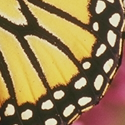
\includegraphics[width=0.23\textwidth]{imgs/img_003_true_crop.png}\hspace{-0.75cm}
	\label{fig1:subfig1}}
	\qquad
\subfloat[bicubic]{
	
\includegraphics[width=0.23\textwidth]{imgs/003_bicubic_crop.png}\hspace{-0.75cm}
	\label{fig1:subfig2}}
	\qquad
\subfloat[SRCNN]{
	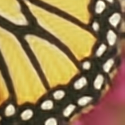
\includegraphics[width=0.23\textwidth]{imgs/img_003_SRCNN_crop.png}\hspace{-0.75cm}
	\label{fig1:subfig3}}
	\qquad
\subfloat[DRCN]{
	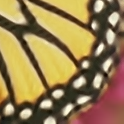
\includegraphics[width=0.23\textwidth]{imgs/img_003_Kim_crop.png}
	\label{fig1:subfig4}}\\[-2ex]

\subfloat[Main, Zero-Pad]{
	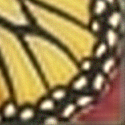
\includegraphics[width=0.23\textwidth]{imgs/img_003_net01_crop.png}\hspace{-0.75cm}
	\label{fig1:subfig5}}
	\qquad
\subfloat[Upscale only]{
	
\includegraphics[width=0.23\textwidth]{imgs/img_003_net02v2_crop.png}\hspace{-0.75cm}
	\label{fig1:subfig6}}
	\qquad
\subfloat[Two-step]{
	
\includegraphics[width=0.23\textwidth]{imgs/img_003_net02_crop.png}\hspace{-0.75cm}
	\label{fig1:subfig7}}
	\qquad
\subfloat[Deep Net]{
	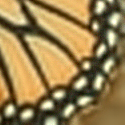
\includegraphics[width=0.23\textwidth]{imgs/img_003_net04_crop.png}
	\label{fig1:subfig8}}\\[3ex]


\subfloat[ground truth]{
	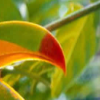
\includegraphics[width=0.23\textwidth]{imgs/img_002_true_crop.png}\hspace{-0.75cm}
	\label{fig1:subfig9}}
	\qquad
\subfloat[bicubic]{
	
\includegraphics[width=0.23\textwidth]{imgs/002_bicubic_crop.png}\hspace{-0.75cm}
	\label{fig1:subfig10}}
	\qquad
\subfloat[SRCNN]{
	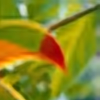
\includegraphics[width=0.23\textwidth]{imgs/img_002_SRCNN_crop.png}\hspace{-0.75cm}
	\label{fig1:subfig11}}
	\qquad
\subfloat[DRCN]{
	
\includegraphics[width=0.23\textwidth]{imgs/img_002_Kim_crop.png}
	\label{fig1:subfig12}}\\[-2ex]

\subfloat[Main, Zero-Pad]{
	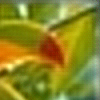
\includegraphics[width=0.23\textwidth]{imgs/img_002_net01_crop.png}\hspace{-0.75cm}
	\label{fig1:subfig13}}
	\qquad
\subfloat[Upscale only]{
	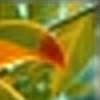
\includegraphics[width=0.23\textwidth]{imgs/img_002_net02v2_crop.png}\hspace{-0.75cm}
	\label{fig1:subfig14}}
	\qquad
\subfloat[Two-step]{
	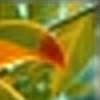
\includegraphics[width=0.23\textwidth]{imgs/img_002_net02_crop.png}\hspace{-0.75cm}
	\label{fig1:subfig15}}
	\qquad
\subfloat[Deep Net]{
	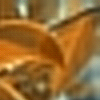
\includegraphics[width=0.23\textwidth]{imgs/img_002_net04_crop.png}
	\label{fig1:subfig16}}


	
\caption{Results of some of our approaches, compared to the ground truth, naive interpolation, SRCNN~\cite{dong2016image} and DRCN~\cite{kim2016deeply}, both images are from the Set5 dataset~\cite{set5}. The upper image is image 003, cropped to the lower right. The lower image is image 002, cropped to the upper right. Zero-padding artefacts can be observed in the first three of our images respectively (e, f, g and m, n, o).}
\end{figure}

\clearpage
\section{Discussion}
Generally we trained our networks for 500 epochs. The training of the main network with repetition padding had to be aborted at 30 epochs because of external circumstances. From the results of this short training we could already see that it removes the border artefacts as expected. Because of that we did not redo the training even though the overall performance was not on par with the other networks yet.

All other networks were trained under the same circumstances and can be compared. It is fairly obvious, that the network without residual skipping failed completely. In fact, the produced pictures were more or less uniformly gray. Thus we see that residual learning is absolutely necessary for our recurrence. Furthermore this explains the vanishing gradients. Most of the output of one recurrent iteration comes from the previous iteration. Only small corrections are caused by the actual network inside. Network parts with small influence always have small gradients too.

According to the results in Table \ref{label:tableResultsSet5} the network variants generally improved the results as expected.
All networks (except for the failed non-residual one) perform better than the bicubic interpolation both according to PSNR and SSIM. They all introduce some artefacts. Because of that, in some cases they look less pleasing than bicubic interpolation even though they produce a sharper image. These artefacts could probably be removed with more training (more epochs and/or bigger data sets).
The two step training only performs slightly better than the upscale part without recurrence. This shows once more, that our recurrence is too hard to train. For better performance it should probably have more inner channels. Sadly we could not test this because of hardware limitations and time.

Looking at our deeper network (Deep Net) we see that it converges much slower than the others, which should come as no surprise. After the same number of epochs the network produces results with insufficient coloration (see Figure \ref{fig1:subfig16}), the PSNR is rather low and the loss is higher than for the other functioning methods. But against our expectation the SSIM is still higher than for some of the other networks, which suggests that the details where better reconstructed. Regarding this and the fact that the gradient norm is still relatively high, we think that given the appropriate time to train, overall this network would perform the best.

For unknown reasons, our PSNR and SSIM metrics do not match those of other papers (mismatching on bicubic interpolation, see table \ref{label:otherWorksMetrics}). It is unclear to us why exactly the metrics do not match. 
We computed the PSNR ourselves and used a reference implementation for SSIM.
When comparing the baseline of \citet{kim2016deeply} to ours, the performance of our networks are acceptable considering the difference in training time (their $\sim$6 days vs our $\sim$1 day).

\newpage
\section{Conclusion}

We construct a network for super resolution. In the architecture of this network we combine two approaches, an auto-encoder like structure for upscaling and a recurrent CNN for refinement. We try different variants of the network to study the influence of its aspects.

Our first finding is that using residual learning in the recurrent part is instrumental to obtain reasonable convergence speed. Another observation is that zero-padding in the convolutional layers leads to artefacts at the borders. This can be avoided by introducing replication-padding layers before the convolutions. We also clearly see that deeper networks converge much slower.

Our method shows an improvement compared to several naive upscaling methods (nearest neighbour, bilinear, bicubic), but it is far from reaching state of the art performance.
The most obvious reason for this is the lack of training time. Additionally we theorise that a deeper network would work better. But again, this would induce some serious augmentation of the computational complexity.

Improvements to our systems could certainly be achieved by conducting a series of experiments to better tune our hyperparameters. But this was not possible to achieve with our limited resources.







\printbibliography[heading=bibintoc]

\end{document}
